\section{Problem 5: Detailed evaluation of trained models}
\begin{enumerate}
	\item
We compute the average loss for all the validation sequences at each time step. The main script has been modified to load a pre-trained model and process the validation model while computing the loss at each time step individually(This is indicated in the script ptb-lm-P5-1.py under "Loss computation", Line 405). The resulting curves for the three models are shown in Figure \ref{fig:5_1}. \\
The loss is clearly larger when the training starts as the model does not have much information about the sequence at hand and cannot predict accurately. As we proceed, all the models should start making better predictions and thus the reduction of the loss. Although the loss fluctuates, it seems to be stabilizing around certain values, of which the RNN loss shows a higher loss while the GRU and Transformer perform similarly to each other but better than RNN. 
\begin{figure}
	\centering
	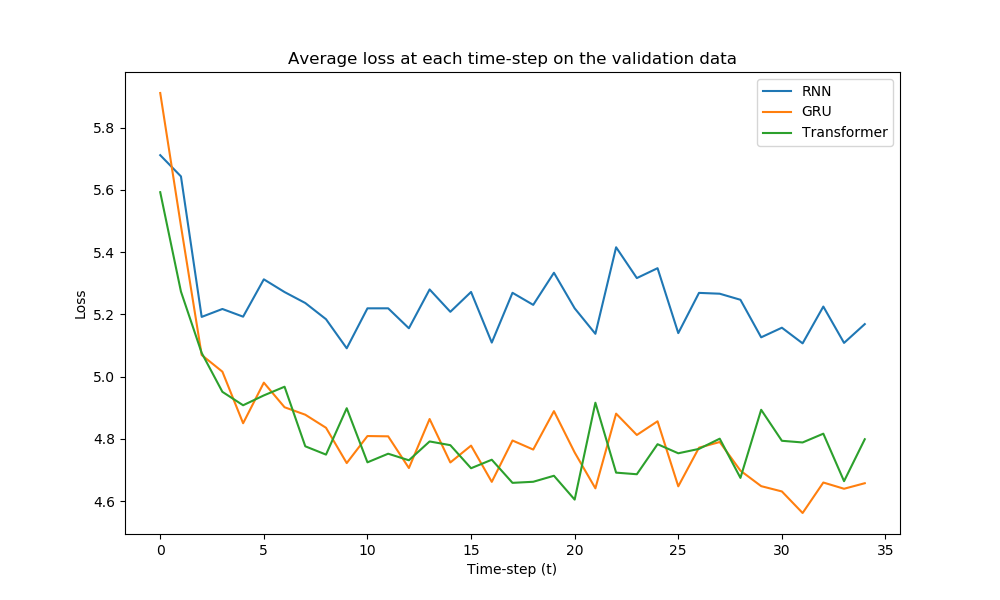
\includegraphics[width=15cm]{loss_t-step}
	\caption{text}
	\label{fig:5_1}
\end{figure}
\item
Similarly to point 1 above, we modified the main script (see ptb-lm-P5-2.py under LOSS COMPUTATION on line 405). Here instead of processing the whole sequence at each step, we only run one mini-batch, processing each time step separately without touching the hidden states. This allows us to compute the gradient at time $T$ with respect to the hidden state at each time step $t$. \\
We compute the norm of the concatenated gradient vectors for the different layers and plot them with respect to the time steps as illustrated in Figure \ref{fig:5_2}. Note that the values for each curve are rescaled to be in the range $[0,1]$. This way we can compare the behavior of the gradients of the two different models (RNN and GRU). The graph shows how the gradients with respect to earlier time-steps are smaller than the gradients with respect to later times. This indicates that long-term dependencies contribute less to the gradient at a given point. The drop in the dependency is particularly steep on the RNN model. On the other hand, the mechanics of GRU help better mainatining the long-term dependencies. 
\begin{figure}
	\centering
	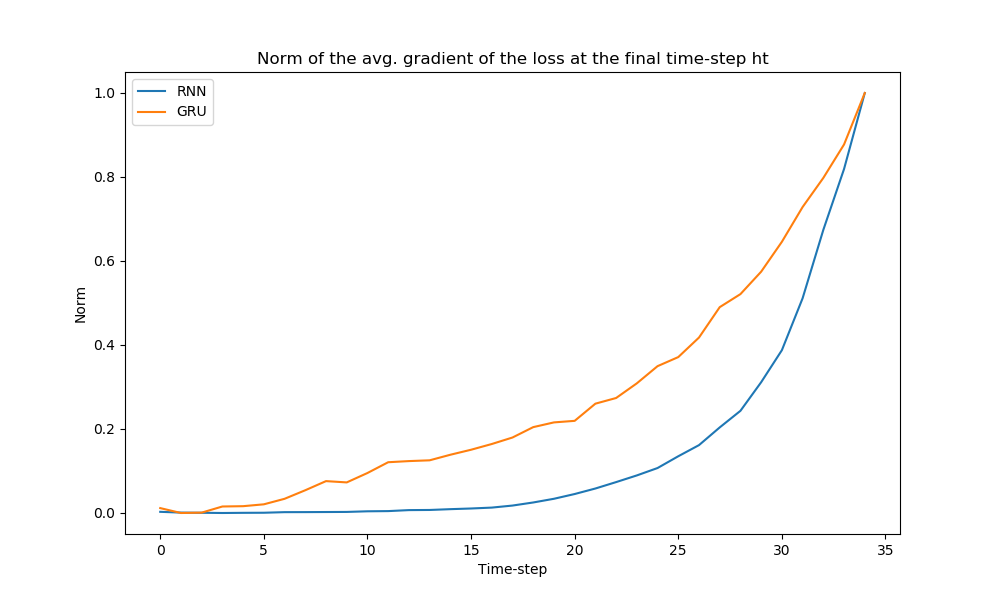
\includegraphics[width=15cm]{gradsL_wrt_ht}
	\caption{text}
	\label{fig:5_2}
\end{figure}
\item
We generate samples from both the simple RNN and GRU. We use the models from section 4.1. The sampling code can be found in the script generate.py. We produce 20 samples from RNN and GRU, 10 samples of the same length as the training sequnences (35) and 10 samples that are twice the length of the training sequeneces (70). The samples can be found in the Appendix of the report. As requested, we choose the three best, worst and interesting samples. The results are declared in the Appendix and can also be found in the provided github repository under folder samples. The subfolders are rnn-35, rnn-70, gru-35, gru-70. 

 
\end{enumerate}